\documentclass{article}
%\usepackage{pgfplotstable,filecontents}
%\pgfplotsset{compat=1.9}% supress warning
\usepackage{graphicx}
\graphicspath{ {img/} }

\title{Gouldboy Color Project Checkpoint (1)}
\author{Maxwell J Svetlik - ms58323}

\begin{document}
    \maketitle

\section{Introduction}
    This is the first report on the Gouldboy Color gameboy emulator project. 
    This brief overview will detail the progress seen over the last checkpoint (which is the proposal), 
    some personal takeaways / gripes, and promised supporting material.
\section{Progress}
    \subsection{CPU Emulation}
    The CPU used by the Gameboy is a modified Zilog z80. Its modified in its instruction set somewhat, but 
    also expands the amount of addressible memory by making the PC and SP registers 16-bit. 
    It is still, however, an 8-bit CPU, though combinations of general purpose registers (which are 8-bit) can be combined 
    to load an effective address.
    \par
    Of the 255 operations described by the architecture, 
    I've implemented all op-codes save the roughly 20 rotate and shift operations. Why have I left these out? 
    Because I'm eager to see visual progress, and they're relatively trivial to implement but take time.
    \par
    Though many of the operations defined are fairly straight forward (most if not all of the 8 and 16-bit ALU ops, etc) 
    and require less thorough testing, some operations are vaguely specified, causing me to make an estimate on their behavior or implementation. 
    Consequently, I've erred on the side of making general purpose functions to handle common aspects to these less understood operations, 
    so if in the future I must correct the behavior, one fix will affect many operations. 
    Some examples of these operations can be found in the project journal entries.
    In the long term, I expect this to impact performance. 
    \par 
    In order to verify cases, I've written an interface that allows the user to place bytes in memory and directly specify the state of the CPU. 
    While using this is tedious to verify instructions, and is by no means thorough, its been written so that 
    it can easily be extended in the future to evaluate written test cases.
    \subsection{The Memory Map}
    \begin{figure}[h]
        \centering
        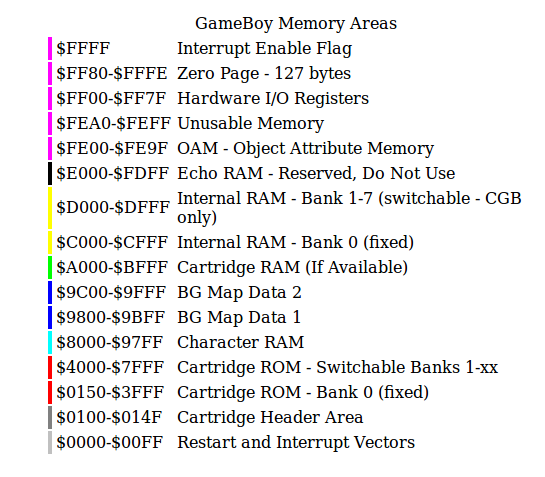
\includegraphics[width=6cm, keepaspectratio]{memmap}
        \caption{A depiction of the gameboy memory map. Courtesy gameboy.mongenel.com}
        \label{fig:memmap}
    \end{figure}
    The memory map of the Gameboy is defined in Figure \ref{fig:memmap}. 
    I talk below about my current interpretation of how the visual system works (which is what I hope to have partially achieved 
    by the next checkpoint). 
    In prepreation for this, I've included skeletons of the hardware timers, and hardward interupt systems.
    As such, I'm right where I predicted for this checkpoint, despite the gripes given in Section \ref{gripes}.
    \section{Takeaways and Knowledge Acquisition}
    \subsection{Regarding the CPU}
    Implementing CPU operations was fairly straightforward. 
    An interesting aspect, and the more challenging part of the implementation, is emulating Gameboy specific hardware. 
    Among other things, this includes things like the Memory Controllers.
    The Memory Controllers are interesting in that, though there is 64kB of addressable memory, the game cartidge only has 
    permanent access to 8kB. 
    These 8kB are used for critical game routines that keep the whole thing running, while other 4kB and 8kB \textit{banks} are swapped 
    out in chunks as needed. 
    This would hold sprites and other visual information relevant to where the player is in the game.
    The controllers facilitate swapping these banks.
    \par
    What I've gleaned about visual output is that the screen buffer is contained within the memory map at specified addresses. 
    This is actually an over simplificiation. There are a dozen visual registers contained in the memory map, double if its a 
    Gameboy Color, since the color pallets must be specified. 
    Writing to the screen then happens at about 60Hz and is communicated via interrupts.
    \subsection{Regarding old Specification Manuals} \label{gripes}
    There exists only a single main, comprehensive resource for Gameboy emulation in the form of a fan-made manual \footnote{http://marc.rawer.de/Gameboy/Docs/GBCPUman.pdf}. 
    Written in the early 2000s, it contains "everything you always wanted to know about the gameboy but were afraid to ask".
    Seemingly, other resource exist on the web, but these all seem to copy the main manual.
    \par
    Though it's a valuable resource, and without it I'd be lost, I find some details lacking for more advanced functions (beyond the CPU). 
    For instance, the details on sound emulation span a single page. 
    Gleaning useful information on the visual or timing systems has proven to be a slow process, 
    requiring more broad system knowledge than I expected.
\section{Supporting Materials}
    \subsection{Commit history}
    I couldn't get \LaTeX to play nice with the .csv, so the commit log is included as an auxillery file as \textbf{log.csv}.
    %\pgfplotstabletypeset[col sep=comma, string type,
    % columns={hash, author, commitdate, message},
    %]{log_cp1.csv}

    \subsection{Project Journal}
    Included below are notes taken in the course of implementing the z80 and (partially) the memory map.
    \begin{figure}[h]
        \centering
        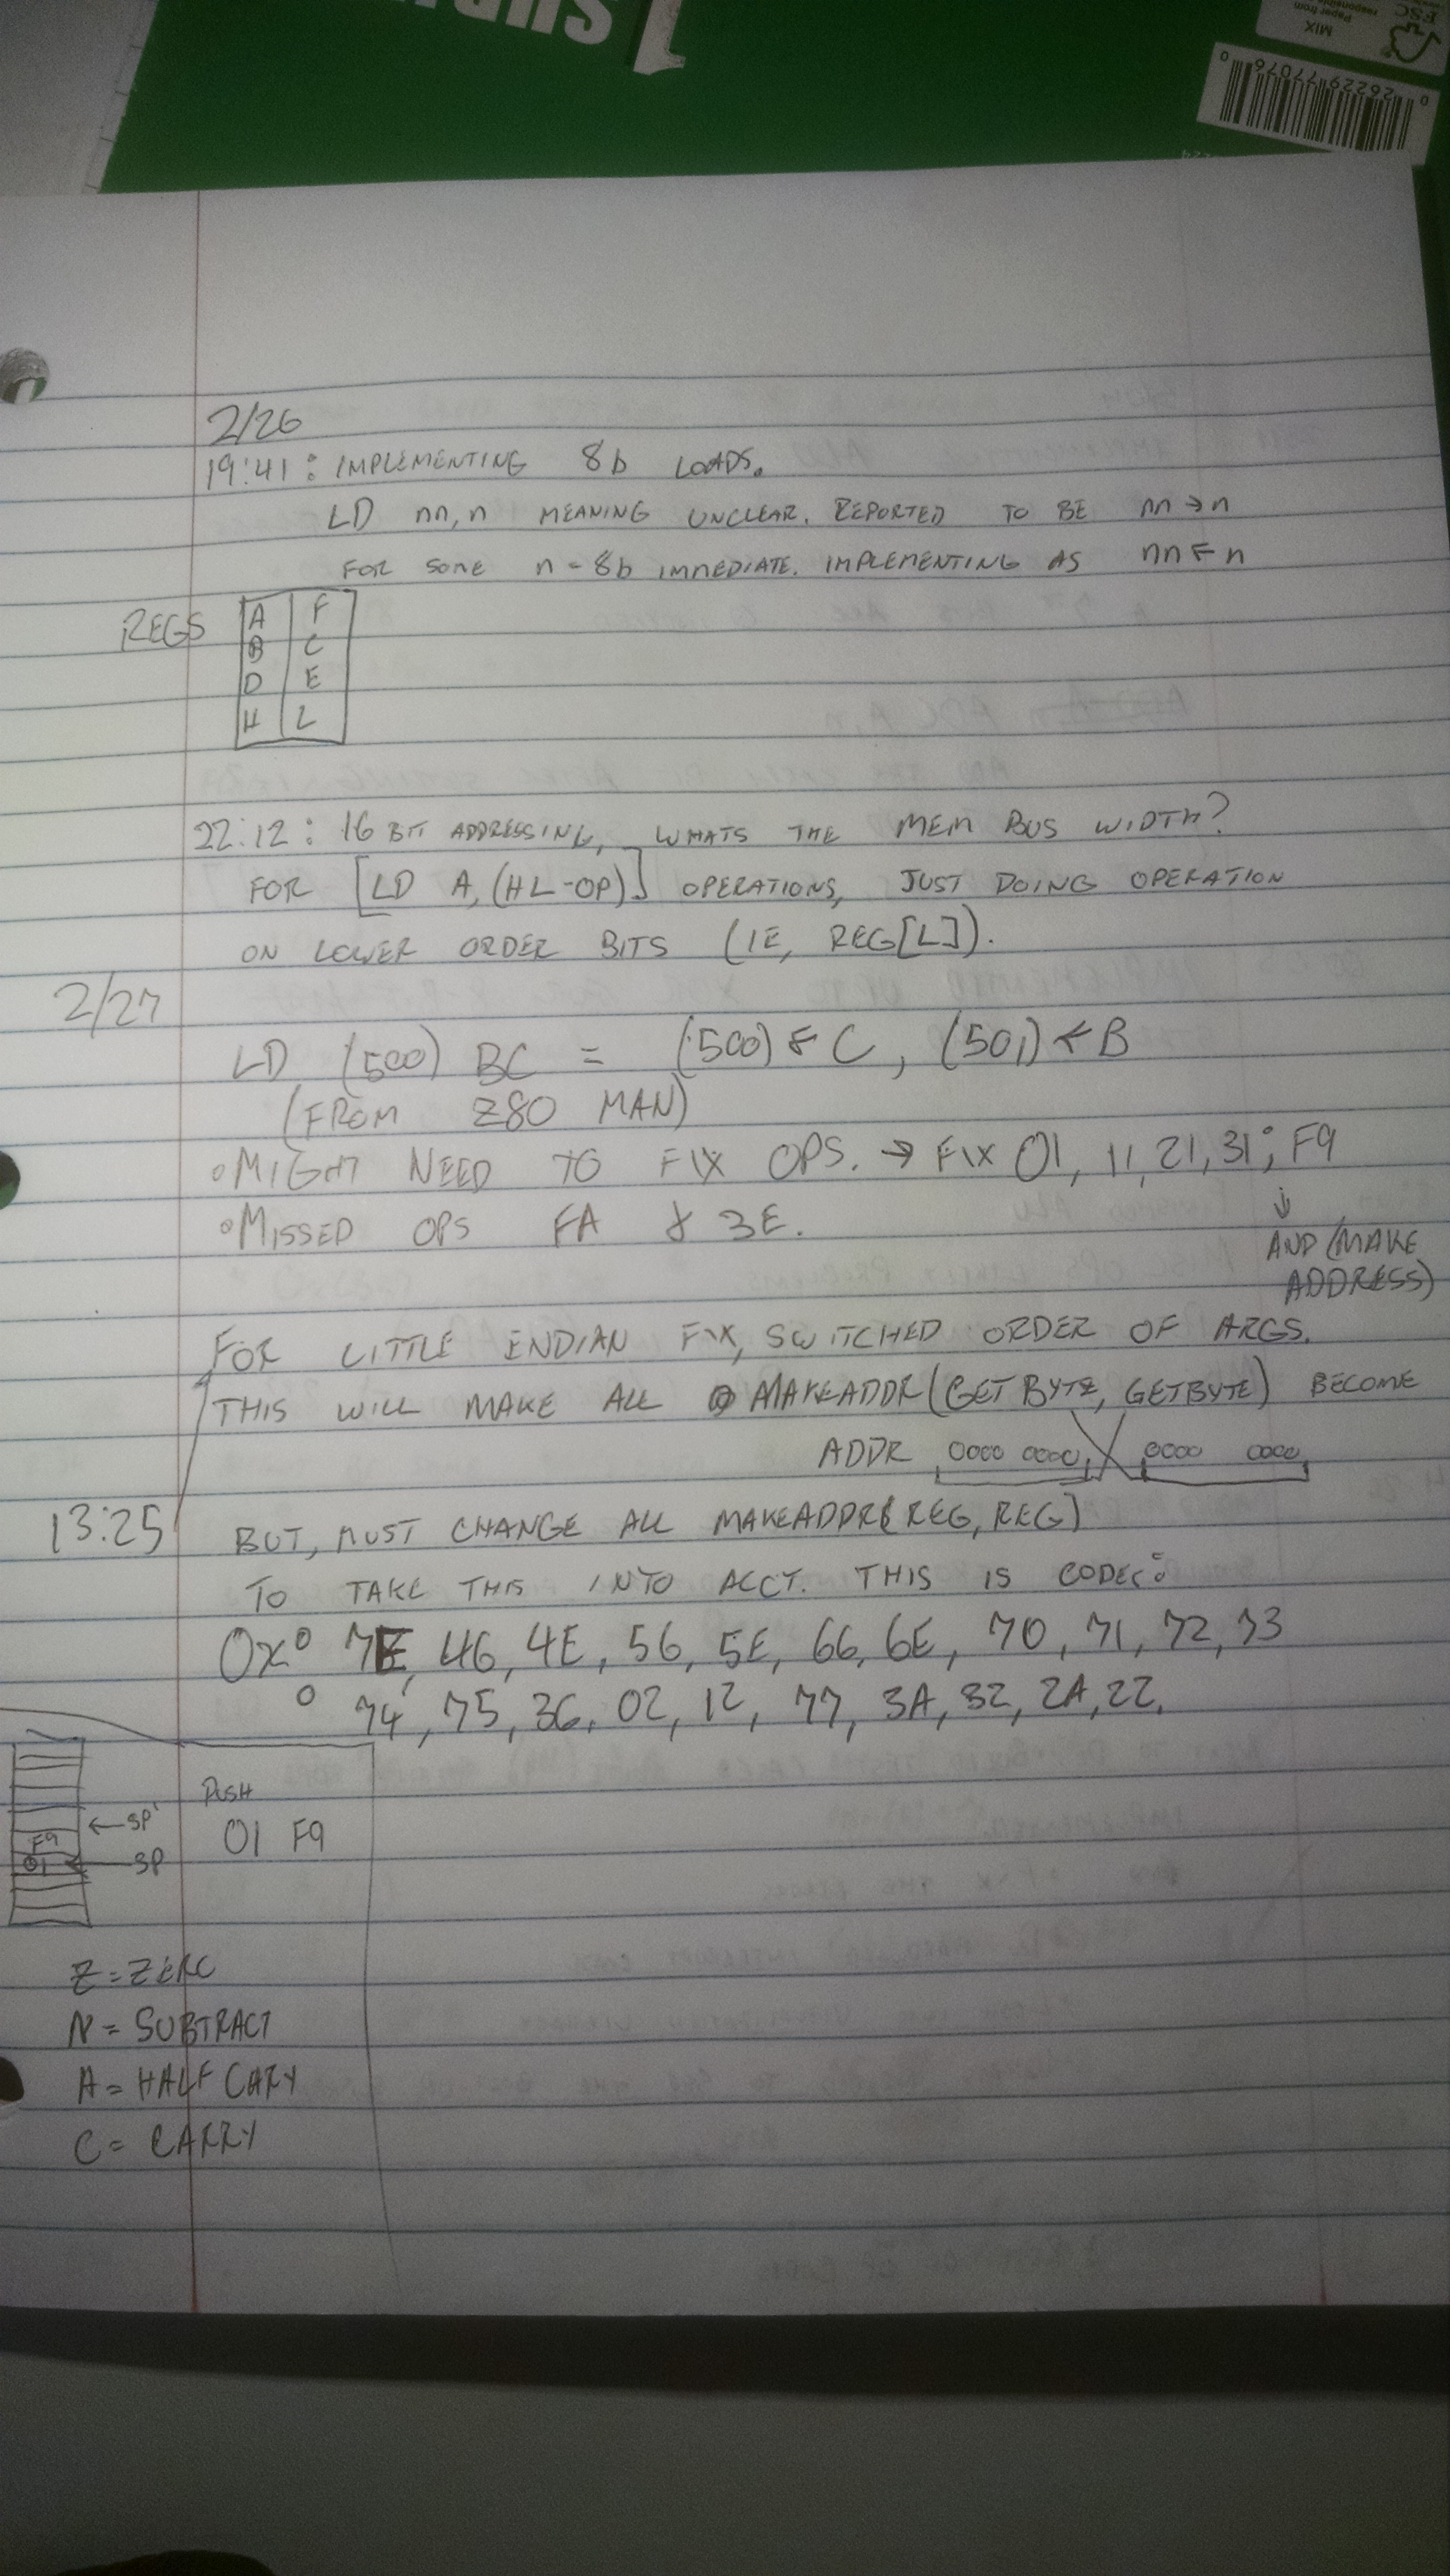
\includegraphics[width=12cm, keepaspectratio]{entry_1}
        \caption{Project entry 1}
    \end{figure}
     \begin{figure}[h]
        \centering
        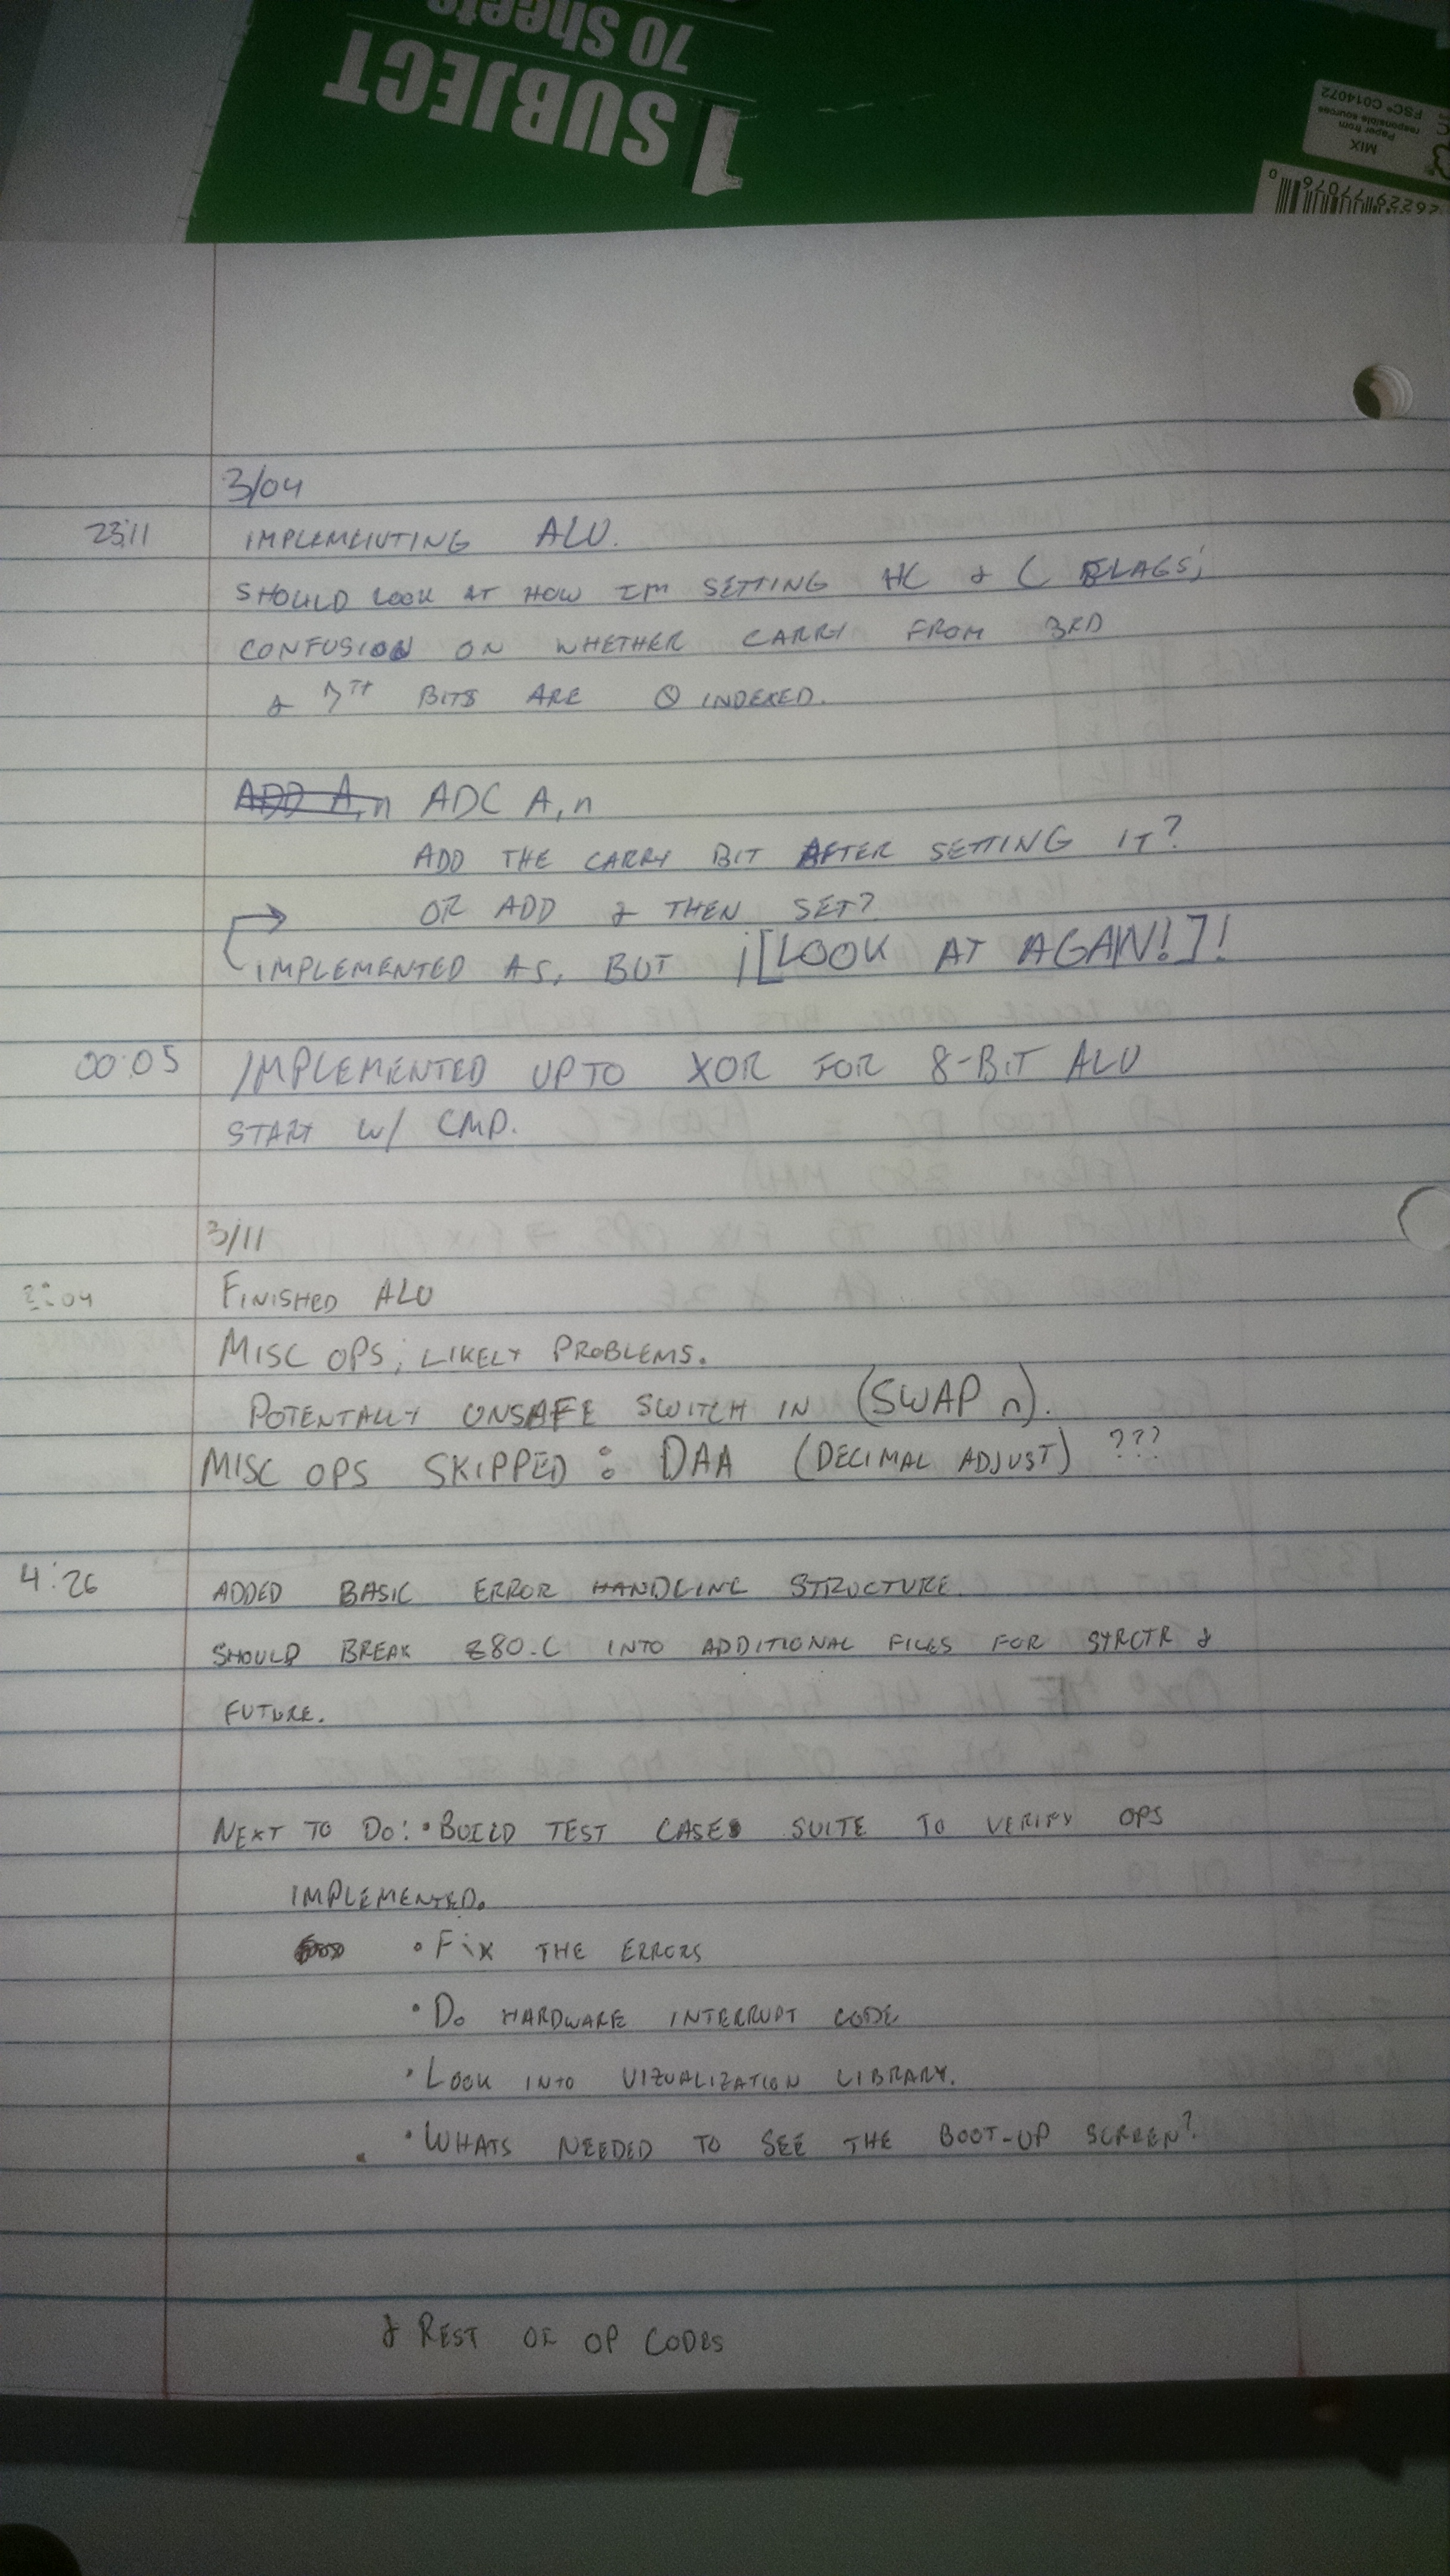
\includegraphics[width=12cm, keepaspectratio]{entry_2}
        \caption{Project entry 2}
    \end{figure}      
    \begin{figure}[h]
        \centering
        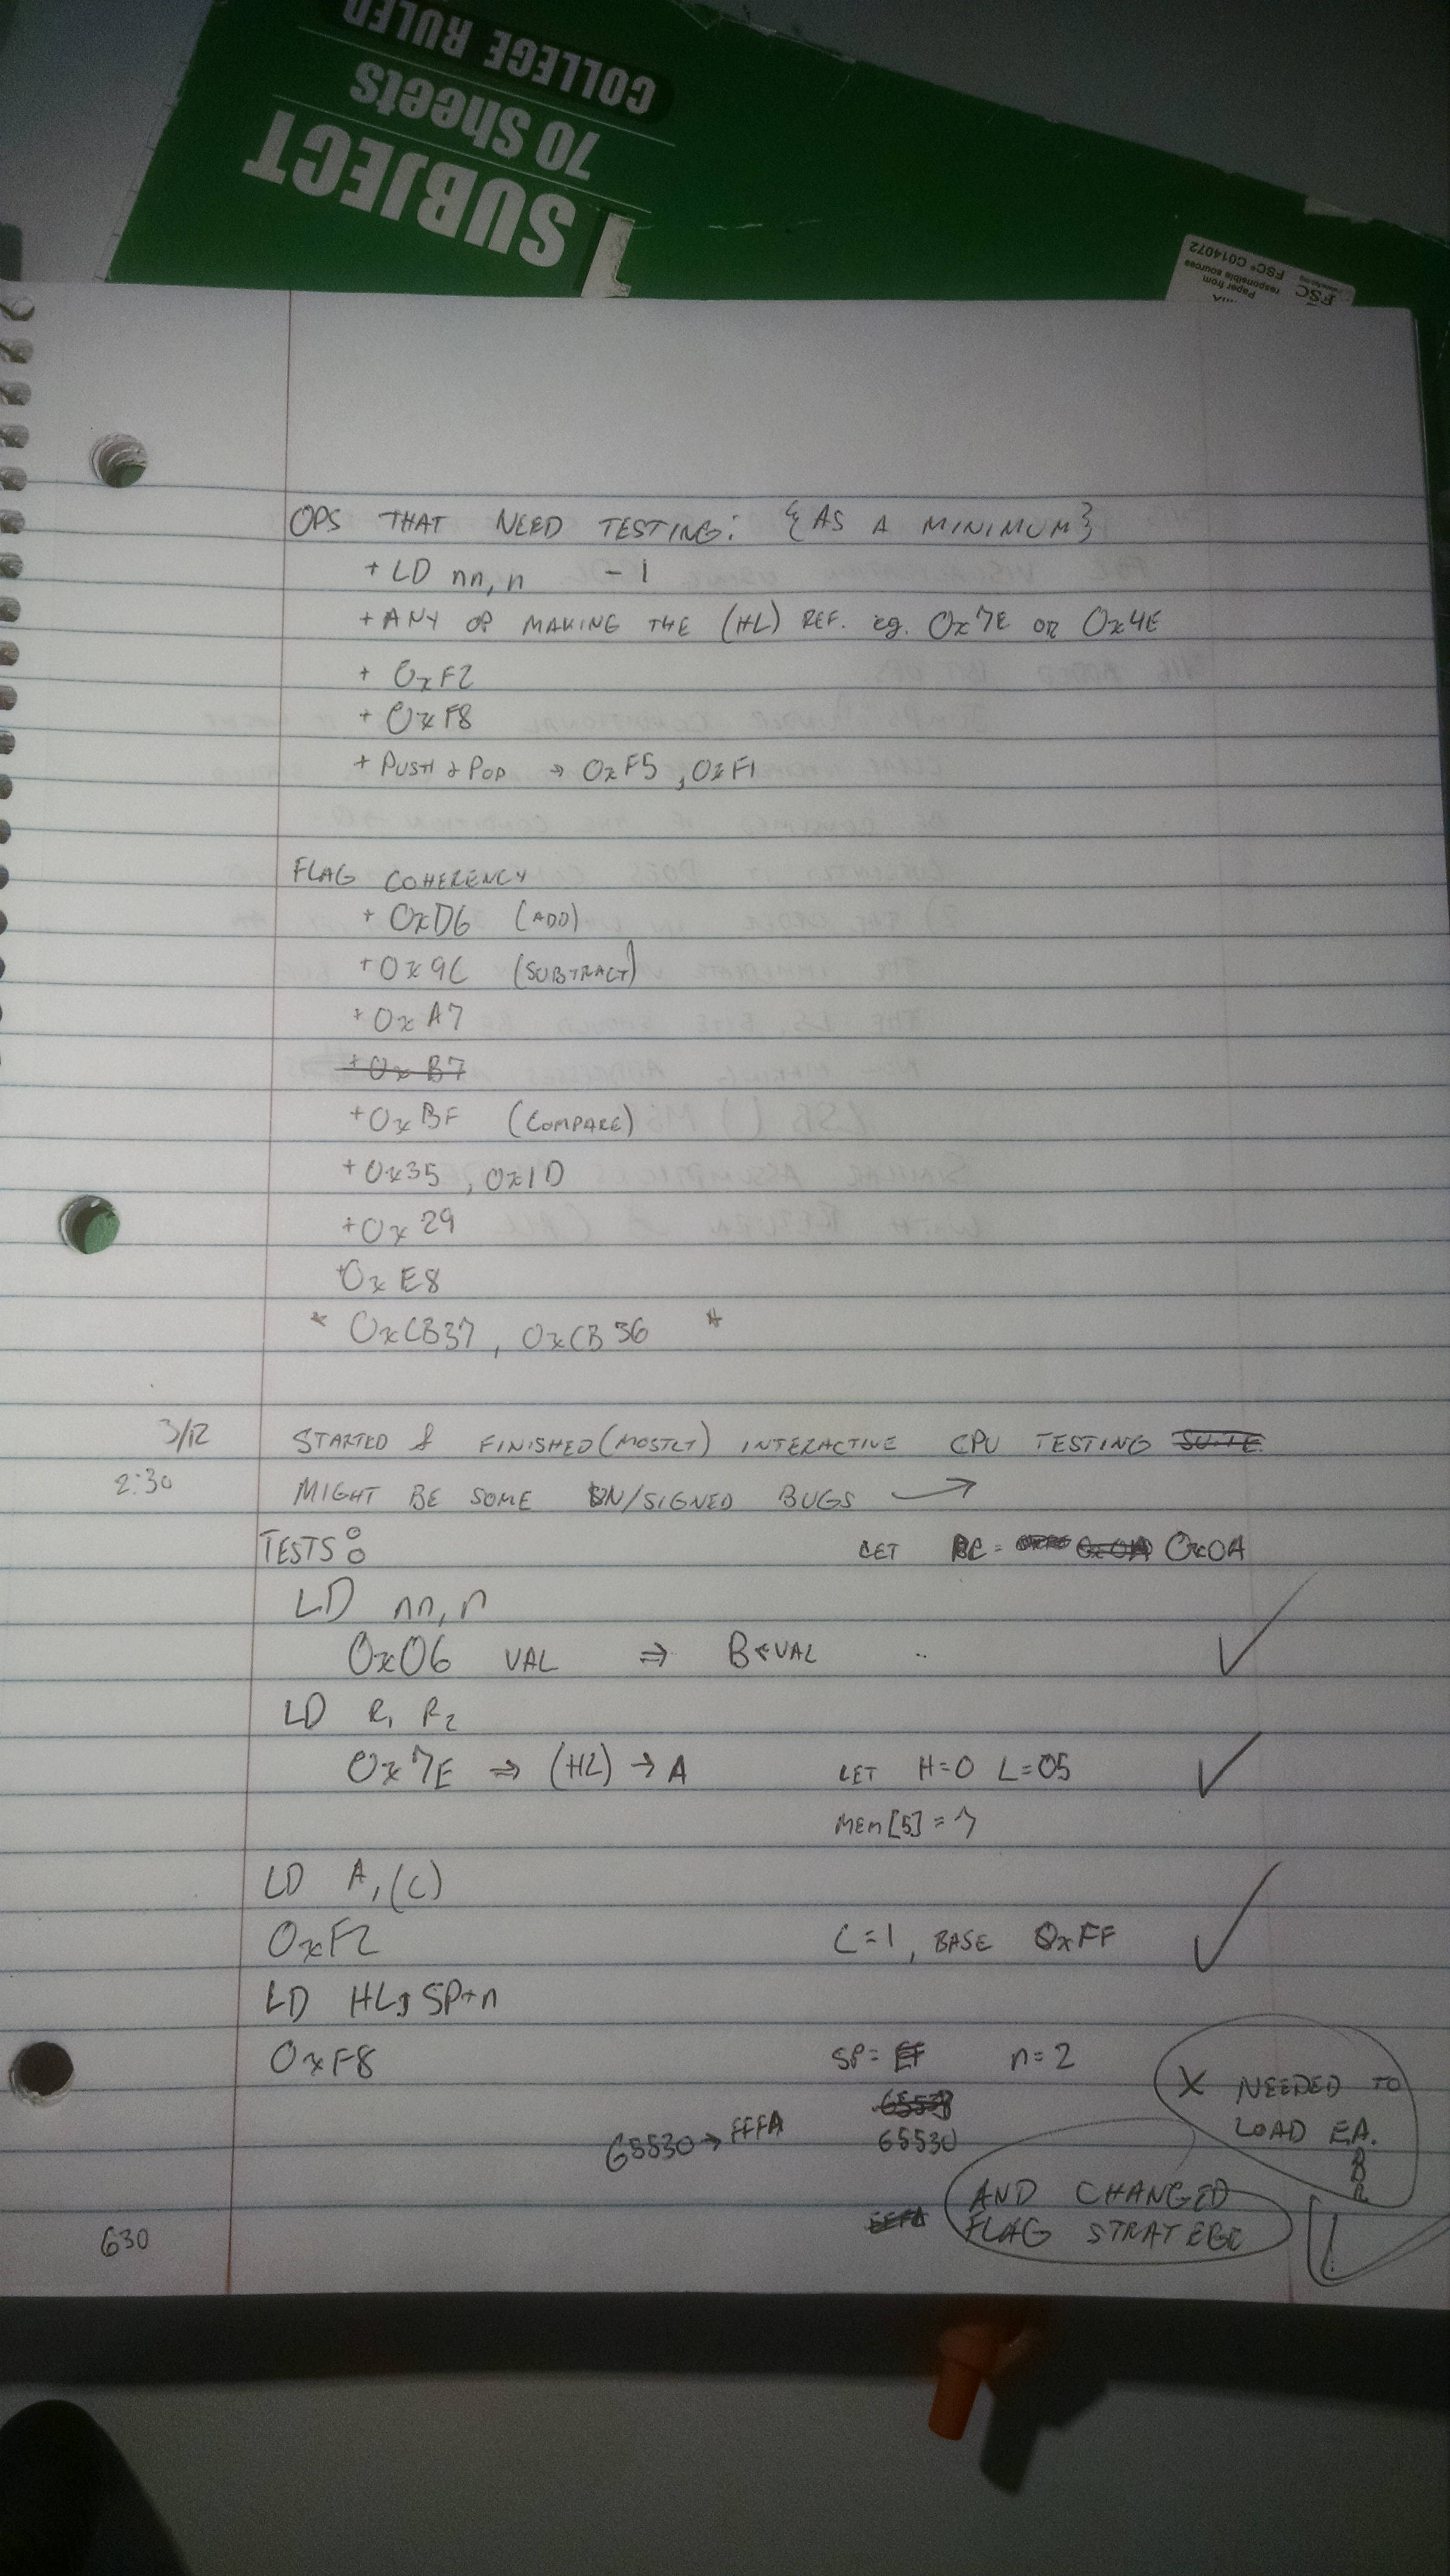
\includegraphics[width=12cm, keepaspectratio]{entry_3}
        \caption{Project entry 3}
    \end{figure}
     \begin{figure}[h]
        \centering
        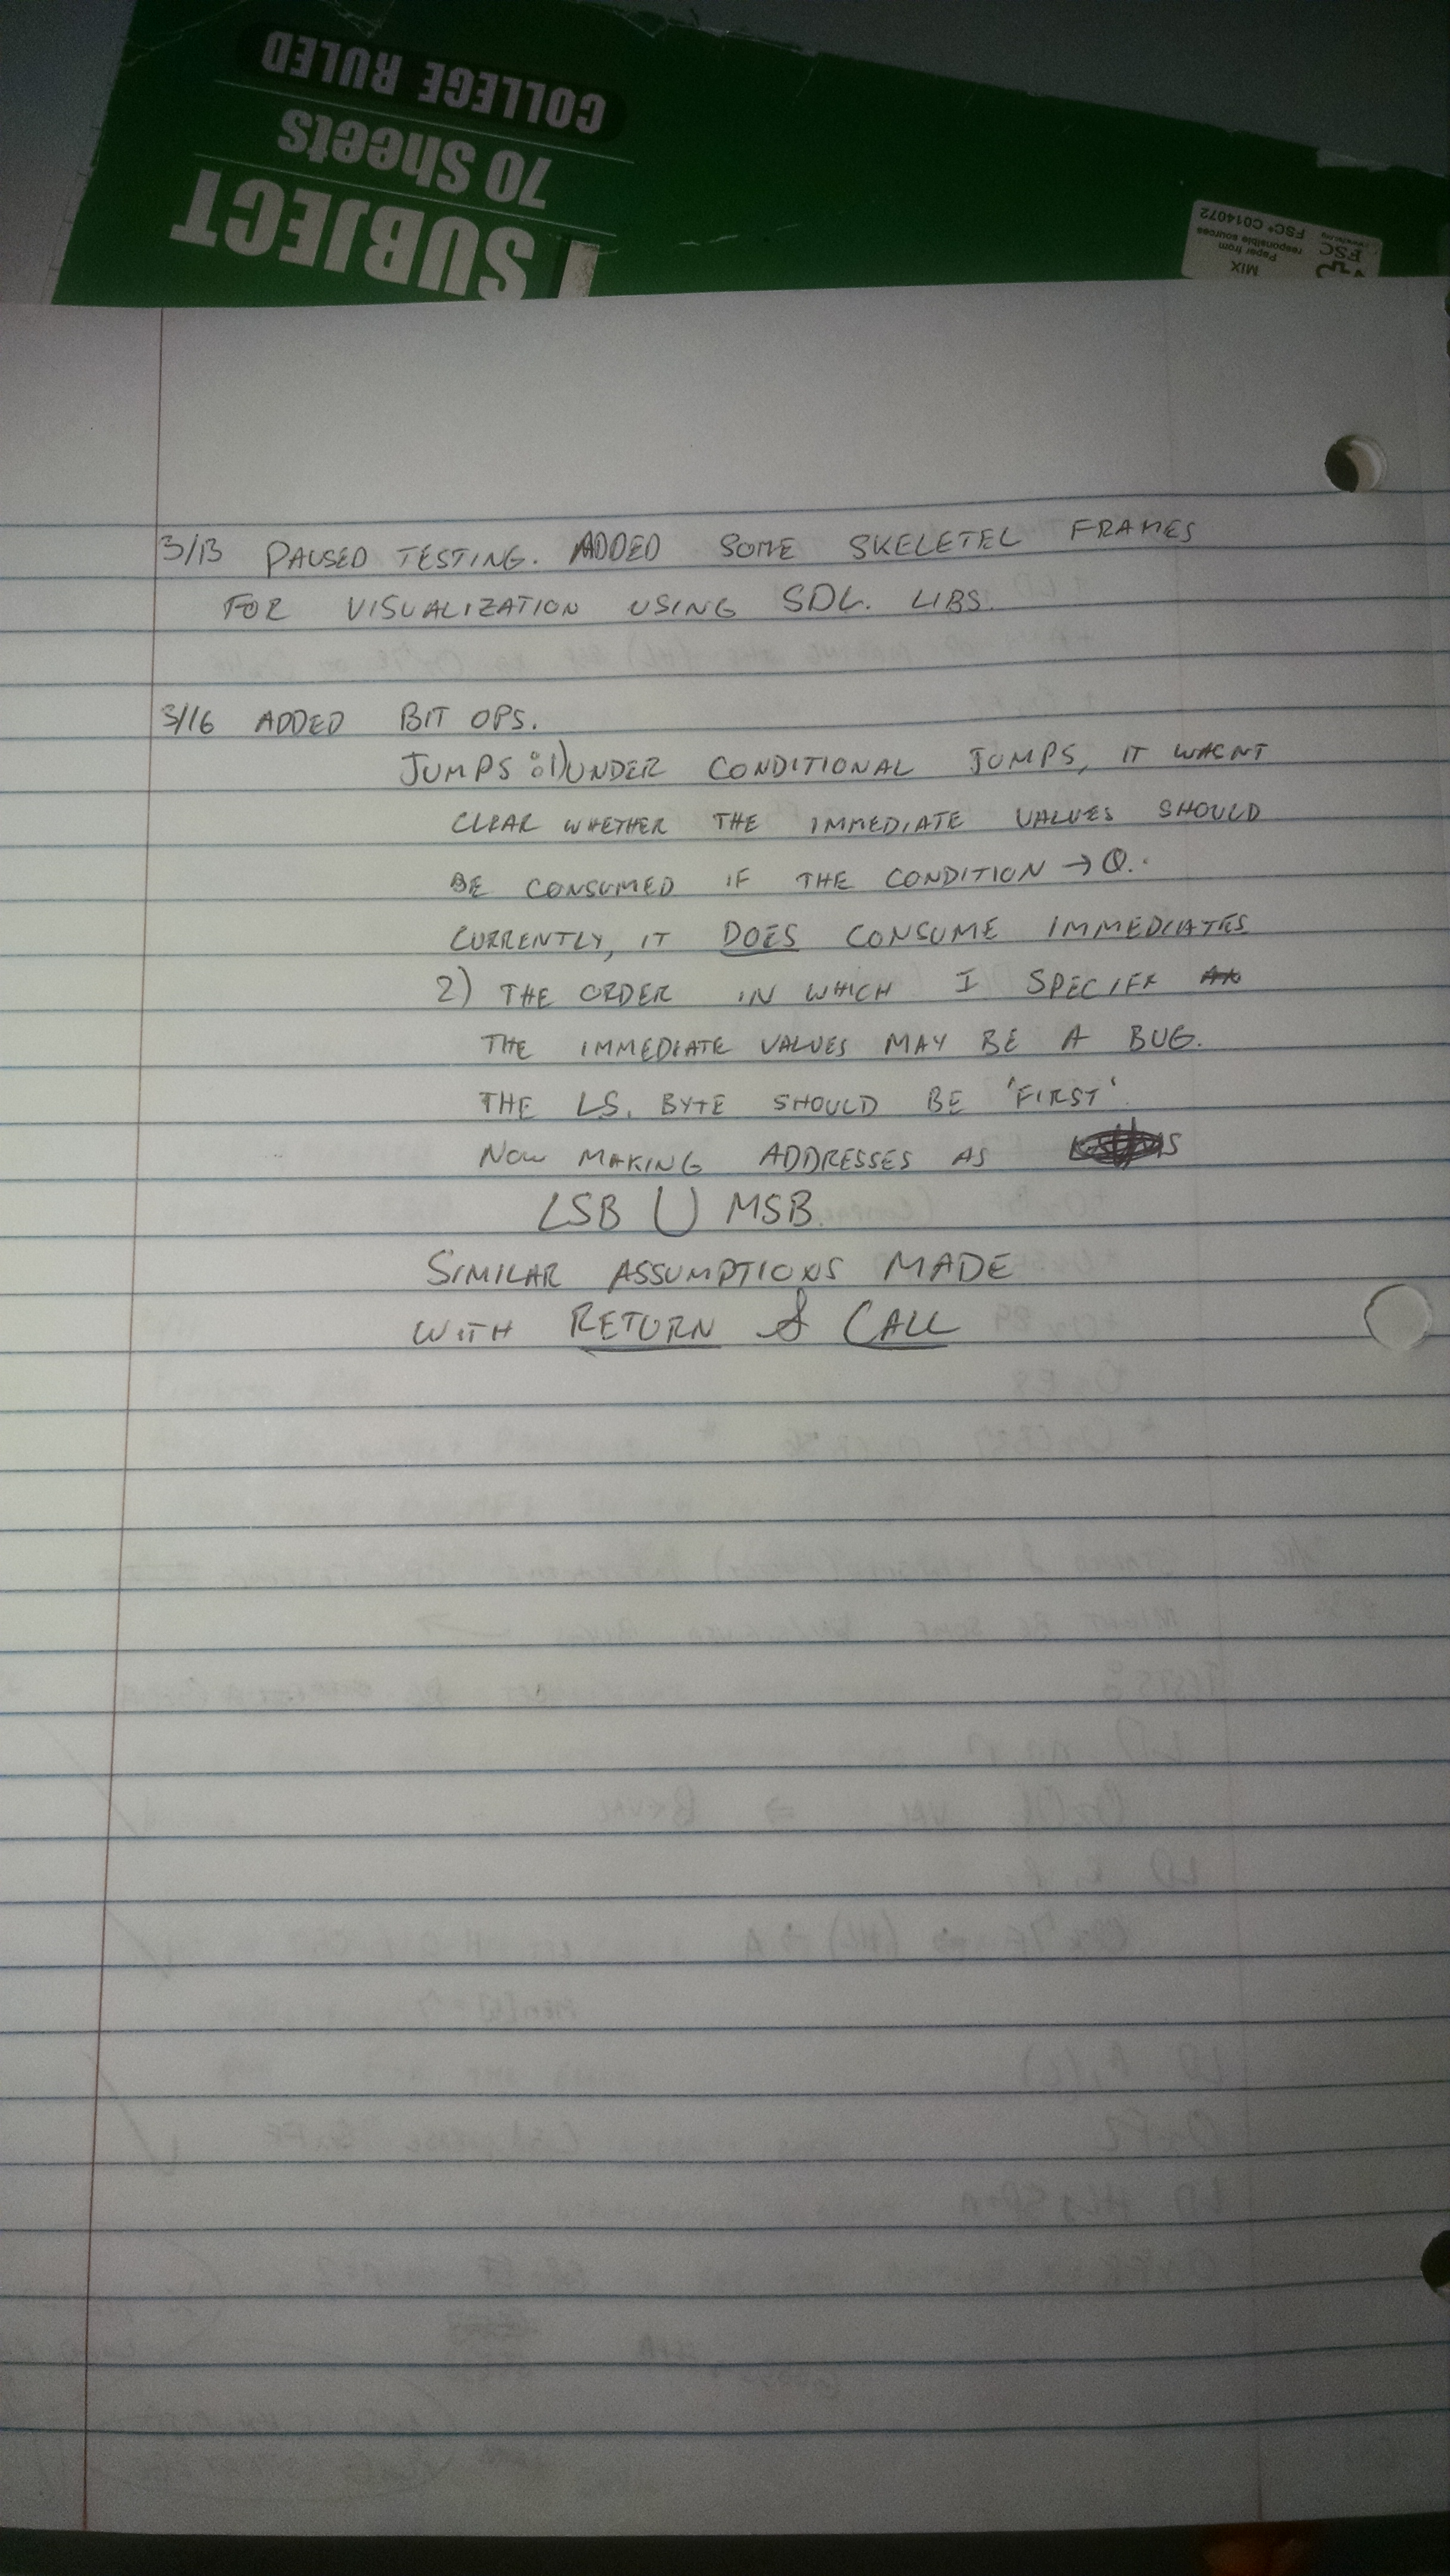
\includegraphics[width=12cm, keepaspectratio]{entry_4}
        \caption{Project entry 4}
    \end{figure}   
    
\end{document}
